\section{Główne metodyki detekcji anomalii}
% Dla zadania detekcji anomalii w celu doboru odpowiedniej metody należy na samym początku rozpatrzyć zbiór odniesienia (opisane w podsekcji \ref{sub:loc_glob}) oraz algorytm, który dokładnie modeluje dystrybucję danych. Większość algorytmów detekcji dla uczenia nienadzorowanego opartych jest na następujących metodach:
Dobór metody do detekcji anomalii jest złożonym zadaniem. Detektor anomalii powinien jak najbardziej separować obserwacje odstające od reszty obserwacji. Zdefiniowanie normalnego obszaru zwierającego wszystkie poprawne obserwacje jest ciężkie do osiągnięcia dla rzeczywistych zbiorów danych. Dodatkowo wybrany model powinien zapewnić interpretację wartości anomalności -- dlaczego obserwacja uważana jest za anomalię. Co pozwala na dalszą analizę obserwacji w celu uzyskania informacji na temat jej powstania anomalii oraz znaczenia dla danego zbioru danych. 
\subsection {Metody oparte na wiedzy statystycznej}
Pierwsze metody detekcji anomalii wywodziły się z analizy statystycznej danych. Popularną metodą jest detekcja anomalii z wykorzystaniem rozkład cechy statystycznej. Analizując rozkład cechy statystycznej, wartości znacząco odstające od średniej wartości (regułą trzech sigm) są wartościami odstającymi (anomaliami). Rysunek \ref{fig:pudleko} przedstawia wykres pudełkowy -- sposób wizualizacji rozkładu cechy -- dla którego wartości poza dolnym i górnym wąsem są wartościami odstającymi. 
\begin{figure}[h!]
    \centering
    \includegraphics[width = 0.39\textwidth]{chapters/istniejace/images/wykres-pudełkowy2-1.png}
    \caption{Wykres pudełkowy z wartościami odstającymi}
    \footnotesize{źródło: \cite{pudelko}}
    \label{fig:pudleko}
\end{figure}

    \subsection {Metody oparte na sąsiedztwie obserwacji}
Metody do wyznaczenia wartości anomalności obserwacji rozpatrują sąsiedztwo (zbiór odniesienia) analizowanej obserwacji. Najbardziej popularne podejścia obliczenia anomalności obserwacji względem sąsiedztwa to:
\begin{itemize}
    \item Wykorzystujące klasteryzację: metoda klasteryzuje dane wejściowe na większe i mniejsze skupienia. Wartość anomalności wyznaczana jest z wykorzystaniem odległości obserwacji do najbliższego dużego skupienia oraz rozmiar klastra, do którego przypisano obserwację.
    \item Wykorzystujące metrykę: wartość anomalności obliczana jest jako długość między obserwacją a k najbliższymi sąsiadami. (Przykład opisany w podsekcji \ref{knn})
    \item Wykorzystujące gęstość: wartość anomalności obliczana jest jako stosunek lokalnej gęstości obserwacji do średniej lokalnej gęstości k sąsiadów. (Przykład opisany w podsekcji \ref{lof})
    \item Wykorzystujące miarę kąta: wartość anomalności obliczana jest na podstawie miary kąta między obserwacją a k sąsiadami. Dla wielowymiarowych zbiorów danych miara kąta jest stabilniejszą metryką. (Przykład opisany w podsekcji \ref{abod})
\end{itemize}
\subsection {Metody oparte na łączeniu klasyfikatorów (zespół klasyfikatorów)}
Wykorzystują podejście budowania silnego klasyfikatora składającego się ze słabszych klasyfikatorów. Główne algorytmy korzystające z podejścia to: \textit{Isolation Forest} oraz \textit{Lightweight Online Detector of Anomalies}. \textit{Isolation Forest} wykorzystuje drzewa decyzyjne do estymacji anomalności obserwacji, natomiast \textit{Lightweight Online Detector of Anomalies} wykorzystuje do tego celu histogramy (algorytmu opisane zostały w podsekcji \ref{iforest} oraz \ref{loda})
\subsection {Metody oparte na sieciach neuronowych}
Podejście wykorzystuje sieci neuronowe do detekcji anomalii. Popularnym rodzajem wykorzystywanych sieci neuronowych są autoenkodery. Jest to jednokierunkowa sieć neuronowe zdolna do rekonstrukcji sygnału wejściowego. Autoenkodery składają się z dwóch elementów: kodera oraz dekodera. Koder przekształca dane wejściowe do niższej wymiarowości, usuwając zbędne informacje, następnie dekoder rekonstruuje dane do wejściowej wymiarowości. Funkcja straty autoenkodera  jest różnicą między danymi wejściowymi a rekonstrukcją danych. Im wyższa funkcja straty tym wyższa anomalność obserwacji.
\begin{figure}
    \centering
    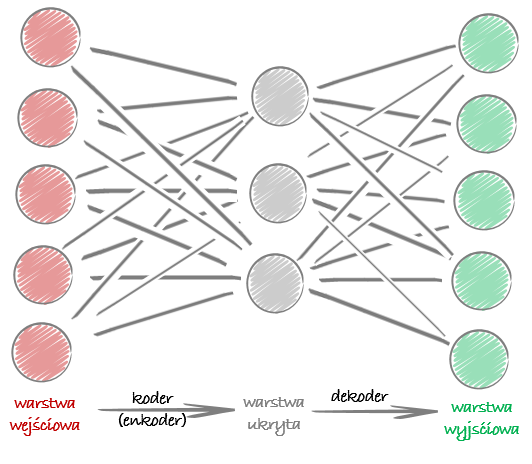
\includegraphics[width = 0.7\textwidth]{chapters/istniejace/images/03-2.png}
    \caption{Budowa autoenkodera}
    \footnotesize{źródło: \cite{ae}}
    \label{fig:pudleko}
\end{figure}
